\section{INTRODUCTION}


In recent years, the technological advances have led to a growing in the availability of massive amounts of continuous streaming data (i.e., event streams) in many application domains such as social networks \cite{mathioudakis2010twittermonitor}, Internet of Things (IoT) \cite{miorandi2012internet}, and Maritime surveillance \cite{patroumpas2015event}. Ability to detect and predict the full matches of a pattern of interest (i.e., sequence of events within the event stream) defined by a domain expert, is important for several operational decision making tasks.
An event stream is an unbounded collection of timely ordered data observations in the form of an attribute tuple that is composed of a value from finite event types along with other categorical and numerical features. In this work we deal with movement event streams, for instance, in the context of maritime surveillance, event patterns prediction over real-time tracking streams of moving vessels is useful to alert maritime operation mangers about suspicious activities (e.g., fast sailing vessels near ports or illegal fishing) before they happen, in this scenario, the event stream of a moving vessel consists of spatial-temporal and kinematic information along with the vessel's identification and its trajectory related events. However, processing real-time streaming data with low latency is challenging since data streams are large and distributed in nature and continuously keep on coming at a high rate. 
% we describe the design and implementation of a system called% 
\par In this paper, we present a design and implementation of an online, distributed and scalable pattern prediction system over multiple massive streams of events. More precisely we consider the event streams related to trajectories of moving objects (i.e., vessels and aircrafts). The proposed approach is based on a novel method that combines the distributed online prediction protocol \cite{dekel2012optimal,kamp2014communication} with the event forecasting with Pattern Markov Chain system \cite{alevizos2017event}, implemented on top of the Big Data framework for stream processing Apache Flink \cite{Flink}. We evaluate our proposed system over  real-word data streams of moving objects, in particular, streams of events related to trajectories of aircrafts and moving vessels, which are provided in the context of the datAcron project\footnote{\url{http://www.datacron-project.eu/}}.

\section{RELATED WORK AND BACKGROUND}
\subsection{Pattern prediction over event streams}
\subsubsection*{Event forecasting with pattern Markov Chains:}

\subsection{Distributed Online Learning}

Distributed online prediction by mini-batch based approach has been proposed in \cite{dekel2012optimal}. Their approach is based on a static synchronization method,  the learners periodically communicate  their local models with a central coordinator unit after consuming a fixed number of input samples/events, in order to  create a global model and share it between all learners. This work has been extended in \cite{kamp2014communication} by introducing a
dynamic synchronization scheme that reduces the required communication by monitoring the variance of the local models from a global reference point. In this paper, we address to use the communication-efficient distributed online learning protocol for event patterns prediction, which is internally based on the Pattern Markov Chain (PMC) predictors. The following section gives a detailed description of the synchronization protocol.
\subsubsection*{Communication-efficient distributed online prediction by dynamic model synchronization:}

Algorithm~\ref{algonline:dol} presents the distributed prediction using the communication-efficient distributed online protocol on both the predictor and coordinator nodes. When a predictor $f\in[k]$ observes an event $e_i$ before synchronization phase $t$, it revises its internal state . Note that $m_t$ is the aggregated model received from the coordinator at synchronization phase $t$ and $m_{t+i}$ is the updated local model after observing the $i^{th}$ event in the new batch.

\begin{algorithm}
	\caption{communication-efficient distributed online prediction protocol} 
	\begin{algorithmic}[1] 
		\Statex  {Predictor $f$:} at observing event $e_i$
		\Statex \Indp update model $m_{t+i,f}$ and predict $I$

		\Statex \If {$i\mod b = 0\ and \|m_i - r\|^2 > \bigtriangleup$}  
		\Statex send $m_{t+i,f}$ to Coordinator 
		\Statex \Indm \Indm \textbf{Coordinator} at synchronization:
		\Statex \Indp Receive local models $\{m_{t,f}\}_{f=1}^k$ 	
		\Statex  compute the global model $m$ 
		\Statex send m to all the predictors $[k]$ and set $m_{f,1}\dots, m_{f,k}=m$
	\end{algorithmic}
	\label{algonline:dol}
\end{algorithm}


Moreover, the communication-efficient distributed online learning framework has been extended to handle kernelized online learning models \cite{kamp2016communication}.

\subsection{Technological Background}
In the last years, many systems for large-scale and distributed stream processing have been proposed, including Spark Streaming \cite{Spark},  Apache Storm \cite{Storm} and Apache Flink \cite{Flink}. These framework allow to ingest real-time data streams from different published on distributed message queuing platforms,such as Apache Kafka \cite{Kafka} or  Amazon Kinesis \cite{Kinesis}. We implemented the proposed system over Apache Flink that provides the distributed stream processing components of the distributed predictors, alongside  Apache kafka for streaming the input event streams, and as a messaging platform to enable the distributed online learning functionalities.


\par In the datAcron project, the Flink streaming engine has been chosen as a primary platform for supporting the streaming operations, based on an internal comparative evaluation of several streaming platforms. While The distributed online learning framework has already been implemented in the FERARI \cite{flouris2016ferari}  based on Storm. In Storm, a distributed application is expressed as a so-called "topology", in which the individual processing steps called "Bolts" are connected
in a data workflow. This means, that each Bolt can is sending and receiving data streams from other Bolts, for example, there are bolts generating
the local models for each incoming data streams and there is a Bolt representing the "Coordinator" for executing the synchronization protocol between
the local models. As the synchronization protocol includes the steps of sending the local models to the coordinator (for merging the models) and of sending
the merged model back, it results in a cyclic workflow structure, which is supported in Storm. 

\subsubsection*{Apache Flink:\\}

\par Apache Flink is an open source project that provides a large-scale, distributed and stateful stream processing platform \cite{carbone2015apache}. Flink is one of the recent and common big data processing frameworks, it employees data-stream processing model for streaming and batch data, the batch processing is treated as a special case of streaming applications (i.e., finite stream). The Flink's software stack includes the  $DataStream$ and $DataSet$ APIs for processing infinite and finite data, respectively. These two core APIs built on the top of the Flink's core distributed streaming dataflow engine. Additionally, Flink provides libraries such as Complex event processing for Flink (Flink-CEP), Machine Learning for Flink (FlinkML) and Flink Graph API (Gelly) \cite{carbone2015apache}.

\par The main data abstractions of Flink are $DataStream$ and $DataSet$ that represent read-only collection of data elements. The list of elements is bounded (i.e., finite) in $DataSet$, while it is unbounded (i.e., infinite) in the case of $DataStream$. The Flink's core is a distributed streaming dataflow engine, with each
Flink program is represented by a data-flow graph (i.e., directed acyclic graph - DAG) that executed by the Flink's engine \cite{carbone2015apache}. The data flow graphs are composed of stateful (state is maintained per partition), parallel operations and intermediate data stream partitions.

\subsubsection*{Apache Kafka:\\}

\par Apache Kafka is scalable, fault-tolerant and distributed streaming framework \cite{Kafka}. It allows to publish and subscribe to arbitrary data streams. Kafka manages the stream records in different categories (i.e., topics) that are partitioned and distributed over the Kafka servers. It provides the ability to publish a stream of records to one or more Kafka topic, to be consumed by applications that can subscribe to one or more topic to read data streams. The stream is distribute and balance between receivers within the same group for the sake of scalability.
  





%The distributed online learning framework has already been implemented in the FERARI  distributed streaming architecture based on Storm. 
%In Storm, a distributed application is expressed as a so-called “topology”, in which the individual processing steps called “Bolts” are connected
%in a data workflow. This means, that each Bolt can is sending and receiving data streams from other Bolts, for example, there are bolts generating
%the local models for each incoming data streams and there is a Bolt representing the “Coordinatior” for executing the synchronisation protocol between
%the local models. As the synchronisation protocol includes the steps of sending the local models to the coordinator (for merging the models) and of sending
%the merged model back, it results in a cyclic workflow structure, which is supported in Storm. 
%
%Why Flink
%In the Datacron project, the Flink streaming engine has been chosen as primary platform for supporting the streaming operations, based on an internal comparative evaluation of several streaming platforms
%regarding functionality and performance. We will discuss in section.. how to implement the required communication structure for the distributed
%online learning framework in Flink.
\section{SYSTEM OVERVIEW}
\subsection{Problem Formulation}
%refine the stream and event pattern %
%define the pattern we deal formally%
% include base line 1 batch size in experemintal results%

We follow the terminology of \cite{luckham2008power,alevizos2015complex,zhou2015pattern} to formalize the problem we tackle. Given a set of \emph{$K$} real-time streams of events $S = \{ s_1,s_2, ..., s_k\}$ as input, which are associated with a set of $K$  objects $O = \{ o_1, ..., o_k\}$. Where each stream $s_i=\langle e_1,e_3,...,e_t,...\rangle$  is a time-ordered sequence of events, these events are connected to a moving object  $o_i \in O$,  $e_t$  refers to the current time event within the unbounded stream, we give the definition of the input event sample as follows:  
\begin{definition}
	Each event is defined as a tuple of attributes $$e_i = (type,\tau,a_1,a_2.....,a_n,id)$$ Where $type$ is the event type attribute that takes a value from a set of finite event types/symbols $\Sigma$, $\tau$ represents the timestamp of the event tuple,  the  $a_1,a_2,...,a_n$ are spatial or other contextual features (e.g., speed); these features are varying from one application domain to another, while the $id$ attribute connects the event tuple to an associated moving object.
\end{definition}

A user-defined pattern $\mathcal{P}$ is given in the form of regular expression over $\Sigma$ (i.e., event types) \cite{alevizos2017event}, and the main goal is to predict the full matches of $\mathcal{P}$ within each event stream $s_i\in S$ in real-time.

\par The setting that is considered in this work is described in the following:\\
A large-scale patterns prediction over multiple input event streams system that  consists of $K=\left\vert{S}\right\vert$ distributed predictor nodes $n_1,n_2...,n_k$, each of which consumes an input event stream $s_i\in S$, and provides an online predication service. Each node $i \in [K]$ handles a single event stream $s_i$ associated with a moving object $o_i \in O$, in addition,  it  maintains a local prediction model $f_i$ for the user-defined pattern $\mathcal{P}$. An online prediction about the future full match of the pattern $\mathcal{P}$ in $s_i$ is provided for each new arriving event tuple. In summary, we have multiple running instances of an online prediction algorithm on distributed nodes for multiple input event streams, each instance provides online predications about a pre-defined pattern of events.  We consider as input a massive event streams that describe trajectories of  moving objects, more specifically, event streams of moving vessels in the context of maritime surveillance.  

The defined pattern $\mathcal{P}$ is monitored over each event stream $s_i$  by a  predictor nodes  $n_i$  that maintains a local prediction model $f_i$, where there is one node for each vessel's event stream.  The prediction model $f_i$ gives the ability to provide an online predictions about when the pattern will be completed in the form of an expected number of future events before a full match does occur.

\subsection{The Proposed Approach}
\par We design and develop a scalable and distributed patterns prediction system over massive input event streams of moving objects. We  exploit the event forecasting with Pattern Markov Chains \cite{alevizos2017event} as the base prediction model (i.e., $f_i$).Moreover,  we propose to enable the information exchange between the distributed predictors/learners of the input event streams, by adapting the distributed online predication protocol \cite{dekel2012optimal,kamp2014communication} to synchronize the prediction models, i.e., Markov transitions probabilities of the Pattern Markov Chain (PMC) predictors.

\par We propose a $synchronization operation$  for the distributed Pattern Markov Chain (PMC) models based on the maximum-likelihood estimation \citep{anderson1957statistical} for the transition probabilities matrix of the underlaying Markov Chain described by: 
\begin{equation}
\label{eq:pi_estim}
\hat{p}_{i,j}=\frac{\sum_{k \in K} n_{k,i,j}}{\sum_{k \in K} \sum_{l \in L} n_{k,i,l}}
\end{equation}


\par Our approach relies on enabling the collaborative learning between the prediction models of  the input event streams. By doing so, we assume that the underlying event streams belong to the same  distribution and share the same behavior (e.g., mobility patterns). We claim that assumption is reasonable in many application domains, for instance, in the context of maritime surveillance, vessels travel through defined routes by International Maritime Organization (IMO). Additionally, vessels have similar mobility patterns in specific areas such as moving with low speed and multiple turns near the ports \cite{pallotta2013vessel,liu2014knowledge}. That allows our system to dynamically construct a coherent global prediction model for all input event streams based on merging its local models.

\par By enabling collaborative learning our approach is imposing an acceleration of learning of the underlying prediction models with less training data, in addition, it provides an improvement of the predictive performance compared to the no-distributed  version of event forecasting with Pattern Markov Chains system. 


\subsection{Distributed Architecture}
\label{sec:architecture}
Our system consumes an aggregated events stream as input\footnote{In practical, the aggregated input events stream is composed of multiple input event streams for multiple moving objects, which are reconstructed bt the system internally.} of large number of moving objects, which is continuously collected and fed into the system. It allows users to register a pattern $\mathcal{P}$ to be monitored over each event stream of a moving object. Output stream consists of original input events alongside with predictions of full matches of $\mathcal{P}$ is outputted to be displayed to the end users. Figure ~\ref{fig:architecture} presents the overview of our system architecture and its main components.      


\begin{figure}[h]

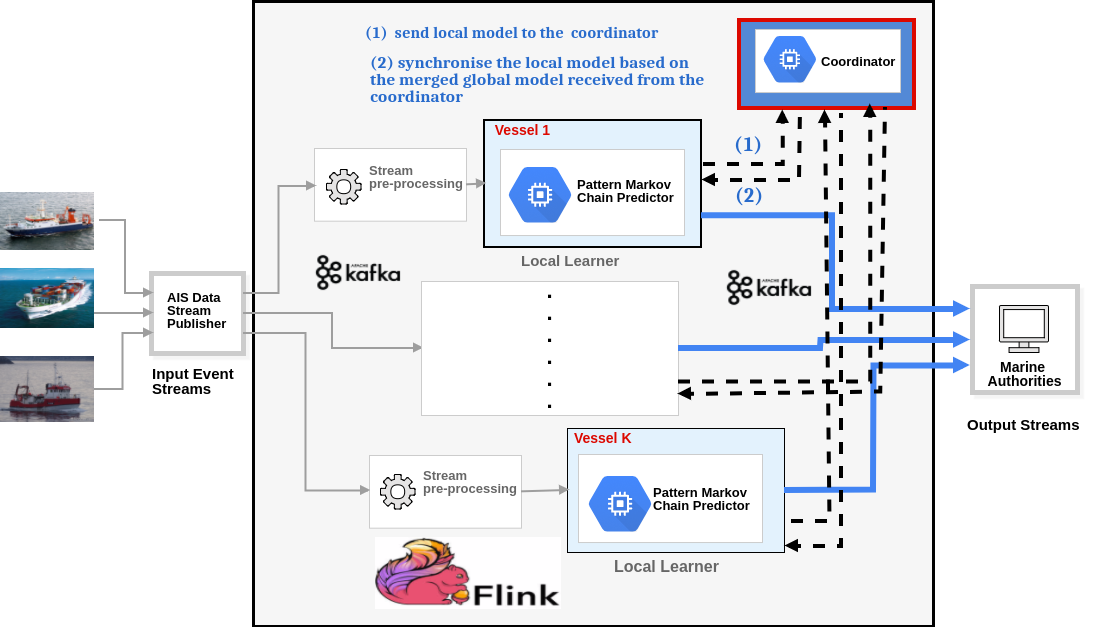
\includegraphics[height=2.5in, width=3.4in]{figures/distributed_architecture.png}
	
\caption{System Architecture.}
\label{fig:architecture}
\end{figure}

The system is composed of three processing units:   \begin{enumerate*}[(i)]
	\item pre-processing operators that receive the input event stream, and perform filtration, ordering operations, before partitioned the input event stream to multiple event streams based on the associated moving object 
	\item predictor nodes (learners), which are responsible to maintain a prediction model for the input event streams, such that each prediction node is configured to handle an event stream from the same moving object, in order to provide online predictions for a predefined pattern $\mathcal{P}$  
	\item a coordinator node that communicates through a Kafka stream channels with the predictors to realize the distributed online learning protocol, which builds a global prediction model based on the received local models, and then share it among the predictors.
\end{enumerate*}

\par In summary, our distributed system consists of multiple pre-processing operators, prediction nodes,  and a central coordinator node. All units are running concurrently and arranged as data processing pipeline as depicted in Figure ~\ref{fig:architecture}. We leverage the Apache Kafka as messaging system to ingest the input event streams and to publish the result streams, in addition, it used as the communication channel between the predictor nodes and the coordinator. While Apache Flink is employed to execute the system's distributed processing units over the input event streams. 

 
\section{IMPLEMENTATION DETAILS}
This sections describes the system's implementation over Apache Flink and Apache Kafka.

\section{EMPIRICAL EVALUATION}
In this section, we present experimental results on real-world event streams in the context of maritime and aviation domains provided by the datAcron project.

\section{CONCLUSION}